\documentclass[addpoints]{exam}
\usepackage{amsmath} % For math.
\usepackage{amsfonts} % For math fonts.
\usepackage{amssymb} % For other math symbols not covered by amsmath.
\usepackage[pdftex]{graphicx} % For pictures, use \includegraphics[scale=decimal]{pic.png}; must be a .png file type.
\usepackage{multicol}
\usepackage{textcomp}
%\usepackage{fullpage}

%\pdfpagewidth 8.5in
%\pdfpageheight 11in

%\setlength\topmargin{0in}
%%\setlength\headheight{0in}
%\setlength\headsep{0in}
%\setlength\textheight{10in}
%\setlength\textwidth{6.5in}
%\setlength\oddsidemargin{0in}
%\setlength\evensidemargin{0in}
%\setlength\parindent{0in}
%\setlength\parskip{.25in}

%\setlength\columnsep{0.3in}

\usepackage{tikz}
\usetikzlibrary{angles,quotes}
\usepackage{tkz-euclide}
%\usetkzobj{all}

\newcommand{\ds}{\displaystyle}
\DeclareMathOperator{\dom}{{dom}}

\def\myrad{3cm}% radius of the circle
\def\myang{60}% angle for the arc

\begin{document}


\begin{flushleft}
Precalculus -  Exam \#3 \hfill  Name: \underline{\hspace{2.5 in}} \\  
  \hfill  Section \# (or meeting time):  \underline{\hspace{1in}}\\  %\hspace{0.0025in} \\
%\hspace*{0.25in} 
Make sure to show all work to receive full credit  \hfill  Score: \underline{\hspace{0.5in}} out of 43 \\
{\bf Important}: Leave all answers as an \underline{\bf exact} value unless otherwise stated.
\end{flushleft}


\begin{questions}


\question
Given the triangle below, evaluate
\begin{parts}
\part[2]  $\tan \theta$.
\part[2] $\sec \theta$.
\end{parts}
\begin{flushleft}

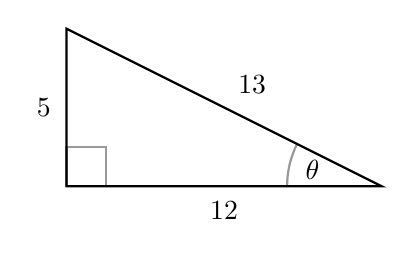
\begin{tikzpicture}[thick]
\coordinate (O) at (0,0);
\coordinate (A) at (4,0);
\coordinate (B) at (0,2);
\draw (O)--(A)--(B)--cycle;

\tkzLabelSegment[below=2pt](O,A){\text{12}}
\tkzLabelSegment[left=2pt](O,B){\text{5}}
\tkzLabelSegment[above right=2pt](A,B){\text{13}}

\tkzMarkRightAngle[size=0.5,opacity=.4](A,O,B)% square angle here
%\tkzLabelAngle[pos = 0.35](A,O,B){$\gamma$}

\tkzMarkAngle[size=1.2cm,%
opacity=.4](B,A,O)
\tkzLabelAngle[pos = 0.9](B,A,O){$\theta$}

\end{tikzpicture}
\end{flushleft}

\question[5] Joule (my other cat) is flying a kite. The kite is extended horizontally 35 feet and flying at an angle of $30^{\circ}$ to the ground.  How high above the ground is the kite?

\vfill

\question[5]  If $\sin \theta=-\frac{\sqrt{2}}{5}$ and $\theta$ lies in quadrant III, find the exact value of $\sec \theta$.

\vfill
\pagebreak
\question[3]  If possible, find the exact value of $\csc^{-1}(2)$.

\vfill

\question[3] Find the exact value of $\sin\left( \dfrac{\pi}{3} \right)$.

\vfill

\question[5] Verify the identity
$$\left(\tan^2 x+1\right)\left(\cos^2 x-1\right)= -\tan^2 x$$

\vfill
\vfill
\pagebreak
\question[5] Find \underline{ALL} the exact solutions of $\sqrt{3} \sec(x) +2=0$

\vfill

\question[5] If possible, write $\tan\left( \sin^{-1}\left(\frac{2}{x}\right)\right)$ as an algebraic expression of $x$.  Hint:  Use a right triangle.

\vfill
\pagebreak
\question[3]  Write an equation for the graph below.\\
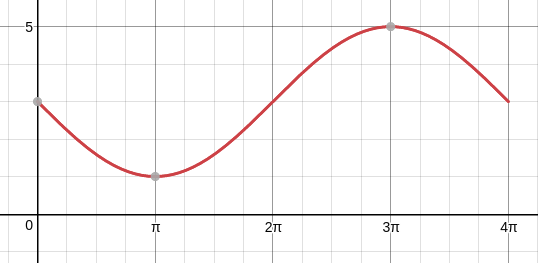
\includegraphics[width=4in]{graph2.png}

\vfill

\question[5] Graph one period of $y=-3\cos\left( \dfrac{\pi}{6}\left(x-2\right) \right)$ in its ``Normal Viewing Window" (Just like in class). Draw at least one intermediate step (or graph) between
your initial graph and final answer.

\hspace*{-0.5in}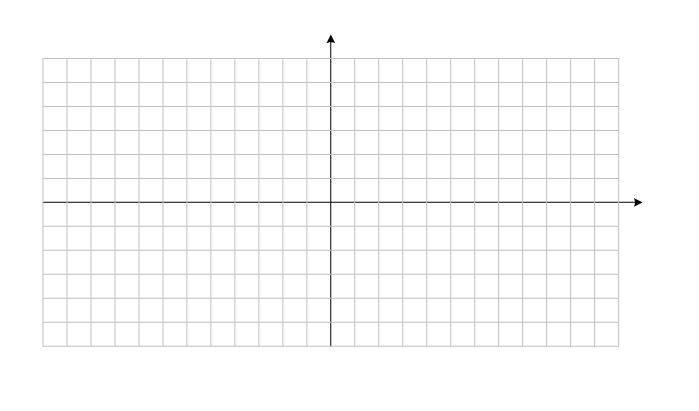
\includegraphics[width=7.5in]{triggrid.png}

\vfill


\end{questions}

\pagebreak

\begin{center}
\LARGE  Formulas
\end{center}


\noindent 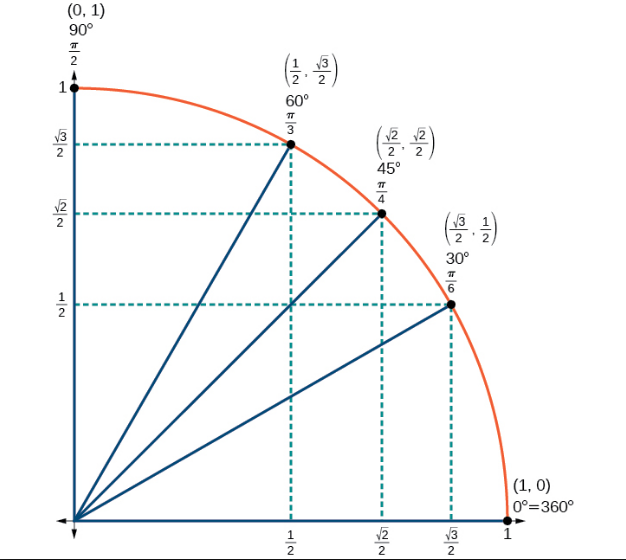
\includegraphics[width=5in]{pic1.png}


\end{document}





























